\documentclass[20pt]{extarticle}
\usepackage{fontspec}
\setmainfont{LiberationSans}[
  Path=fonts/,
  Extension=.ttf,
  UprightFont=*-Regular,
  BoldFont=*-Bold,
  ItalicFont=*-Italic,
  BoldItalicFont=*-BoldItalic
]
\usepackage[paperwidth=594mm,paperheight=841mm,margin=10mm]{geometry}
\pagestyle{empty}
\setlength{\parindent}{0pt}
\usepackage{xcolor}
\usepackage{tcolorbox}
\tcbuselibrary{skins}
\usepackage{graphicx}
\usepackage{booktabs}
\usepackage{array}
\usepackage{enumitem}
\usepackage{tikz}

\definecolor{teal}{HTML}{14505C}
\definecolor{bars}{HTML}{E8B183}
\definecolor{rule}{HTML}{D9B49A}
\definecolor{ink}{HTML}{1B3A3F}

\setlist[itemize]{leftmargin=1.1em,itemsep=0.15em,topsep=0.2em,parsep=0pt}

\newcommand{\sectionbar}[1]{%
  \colorbox{bars}{\makebox[\dimexpr\linewidth-2\fboxsep][l]{\strut\bfseries\color{ink}\fontsize{26}{30}\selectfont #1}}%
}

\newtcolorbox{block}[1]{%
  enhanced, colback=white, colframe=rule, boxrule=0.5pt,
  arc=1mm, left=2.5mm, right=2.5mm, top=1.5mm, bottom=2mm,
  before skip=4mm, after skip=0pt,
  fonttitle=\bfseries,
  title={}, coltitle=ink,
}

\begin{document}

% ---------------------------------------------------------------- header
\begin{tikzpicture}[remember picture, overlay]
  \node[anchor=north west] at ([xshift=10mm,yshift=-8mm]current page.north west)
    {\setlength{\fboxsep}{4mm}\fbox{\parbox[c][14mm][c]{36mm}{\centering\Large\bfseries\color{ink}RI080}}};
\end{tikzpicture}

\vspace*{2mm}
\begin{center}
  {\fontsize{46}{52}\selectfont\bfseries\color{teal}
   Typed Judgment, Deterministic Enforcement:\\[1mm]
   A Consent-Gated Gateway Architecture for Inter-Agent Collaboration over Messaging Channels}

  \vspace{5mm}
  {\Large\color{ink}\bfseries
   Yizhang Cai\textsuperscript{1}\quad Jun Liu\textsuperscript{1}\quad
   Di Ma\textsuperscript{2}\quad Ke Yu\textsuperscript{1}\quad Ke Li\textsuperscript{1}}

  \vspace{3mm}
  \begin{tcolorbox}[enhanced, sharp corners, colback=white, colframe=teal,
    boxrule=0.4pt, width=\textwidth, halign=center,
    borderline={0.4pt}{0pt}{teal,dashed}, fontupper=\normalsize]
    \textsuperscript{1}School of Artificial Intelligence, Beijing University of Posts and
    Telecommunications\quad\textsuperscript{2}Beijing Guoshu Zhilian Technology Co., Ltd.\\
    \texttt{2025111259@bupt.cn}\quad\textbar\quad Special Session XII: Agent Interconnection and
    Collaboration Intelligence
  \end{tcolorbox}
\end{center}

\vspace{2mm}

% ---------------------------------------------------------------- body
% Two flowing columns with the template's seven sections only.

\begin{minipage}[t]{0.482\textwidth}
\vspace{0pt}

\begin{block}{}
\sectionbar{Introduction}
\vspace{2mm}
Messaging channels deliver human events that are unstructured, duplicated,
delayed, or replayed, while agent protocols expect authenticated endpoints,
structured requests, and explicit task state. A gateway must decide whether a
message requests work, which agent is eligible, whether consent is needed, and
whether an event is a replay or an injection.

\vspace{1.5mm}
We separate bounded model judgment from deterministic enforcement: the model
answers seven closed questions (J1 intent, J2 routing, J3 ambiguity, J4 consent,
J5 replay, J6 retryability, J7 injection) and policy code owns thresholds and
every effect.
\end{block}

\begin{block}{}
\sectionbar{Objectives}
\vspace{2mm}
\begin{itemize}
  \item Seven modules from an iMessage/Photon ingress to an ACPs/AIP v2.2
        Leader--Partner path, with four invariants kept in code: authorization,
        identity, isolation, idempotency.
  \item A judgment plane of seven closed questions that returns labels or
        probabilities only and cannot emit free text or call a tool.
  \item Live measurement of routing, consent, the advisory judgment path, and
        the gateway's own handling cost.
  \item A released artifact that reproduces the request suites, the paired
        ablations and the cached judgment responses.
\end{itemize}
\end{block}

\begin{block}{}
\sectionbar{Materials and Methods}
\vspace{2mm}
\textbf{Modules.} M1 ingress authentication; M2 caller/conversation isolation;
M3 discovery and routing; M4 consent; M5 identity-bound execution; M6 state,
idempotency and recovery; M7 delivery and telemetry.

\vspace{1.5mm}
\textbf{Evaluation.} 130 generated requests through the real ingress, three
deliveries each; paired same-code ablations on staging copies; 30 consent trials
plus 10 redeliveries on the deployed adapter; a 280-item judgment suite sampled
three times; a 456-item injection stress set.

\vspace{2mm}
\centering
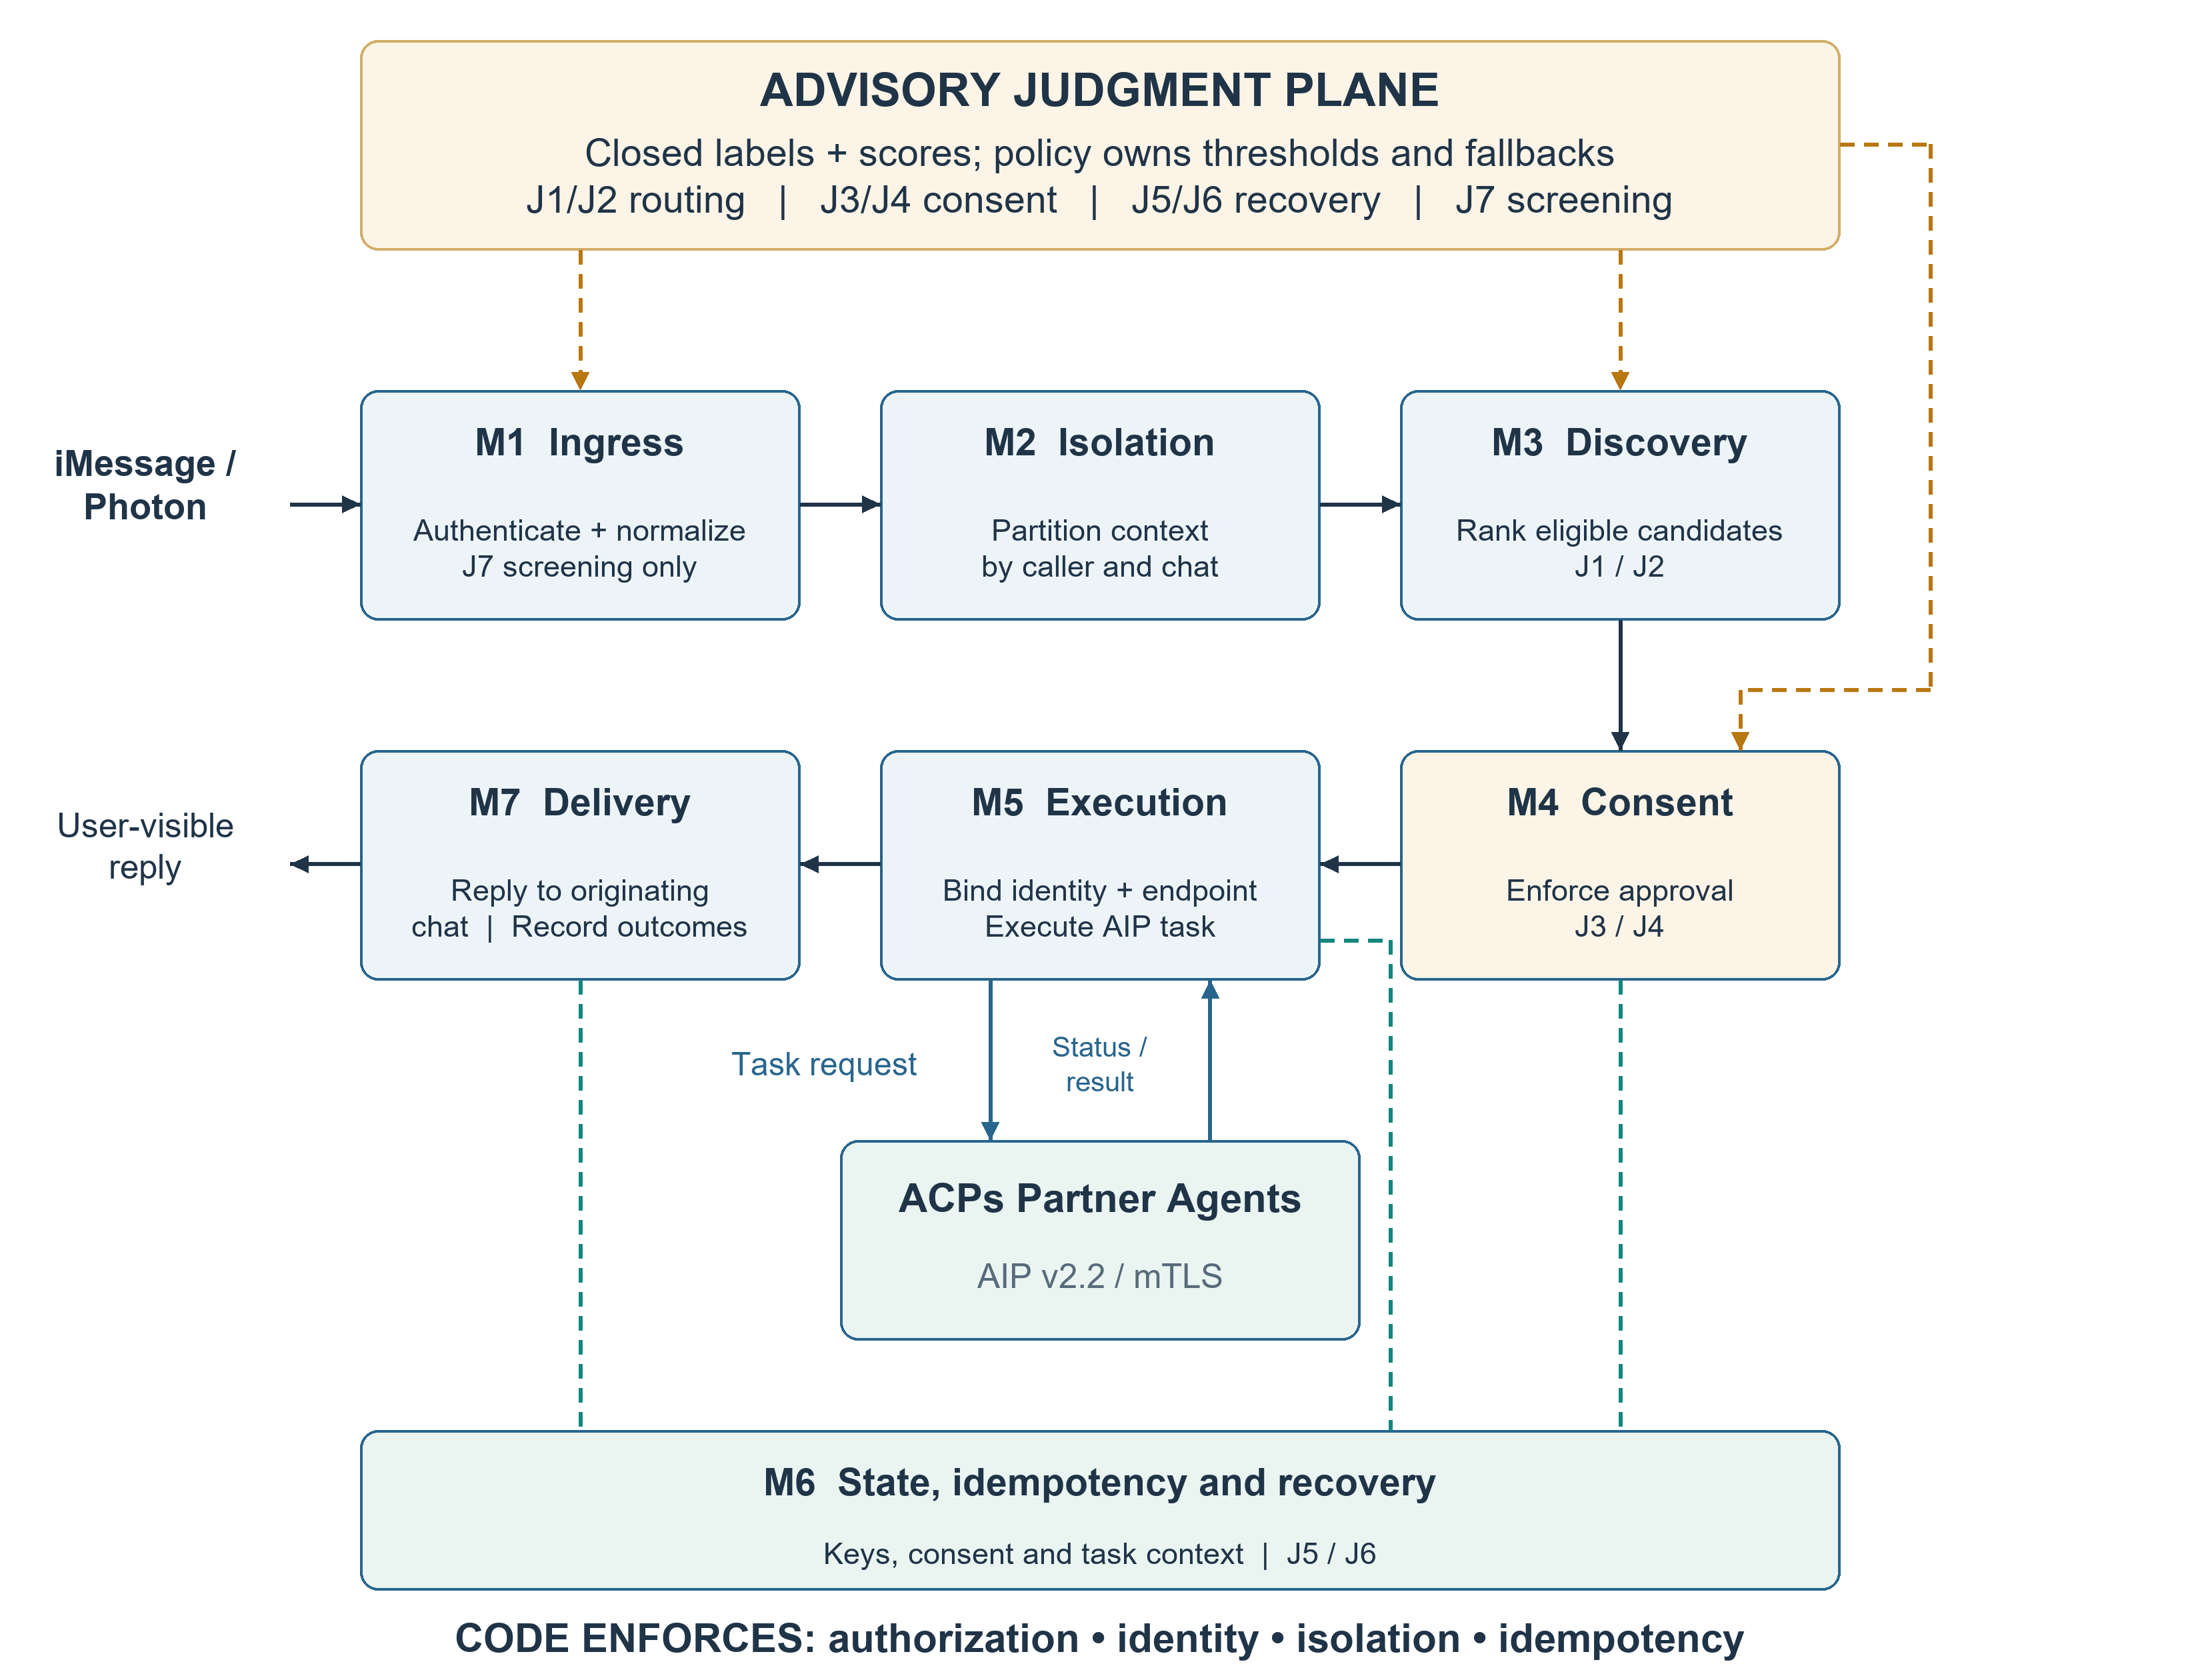
\includegraphics[width=0.85\linewidth]{../figures/fig1_architecture.png}

\vspace{1mm}
\raggedright
\small\textbf{Figure 1.} Seven modules, four invariants, and the advisory
judgment plane.

\vspace{2mm}
\centering
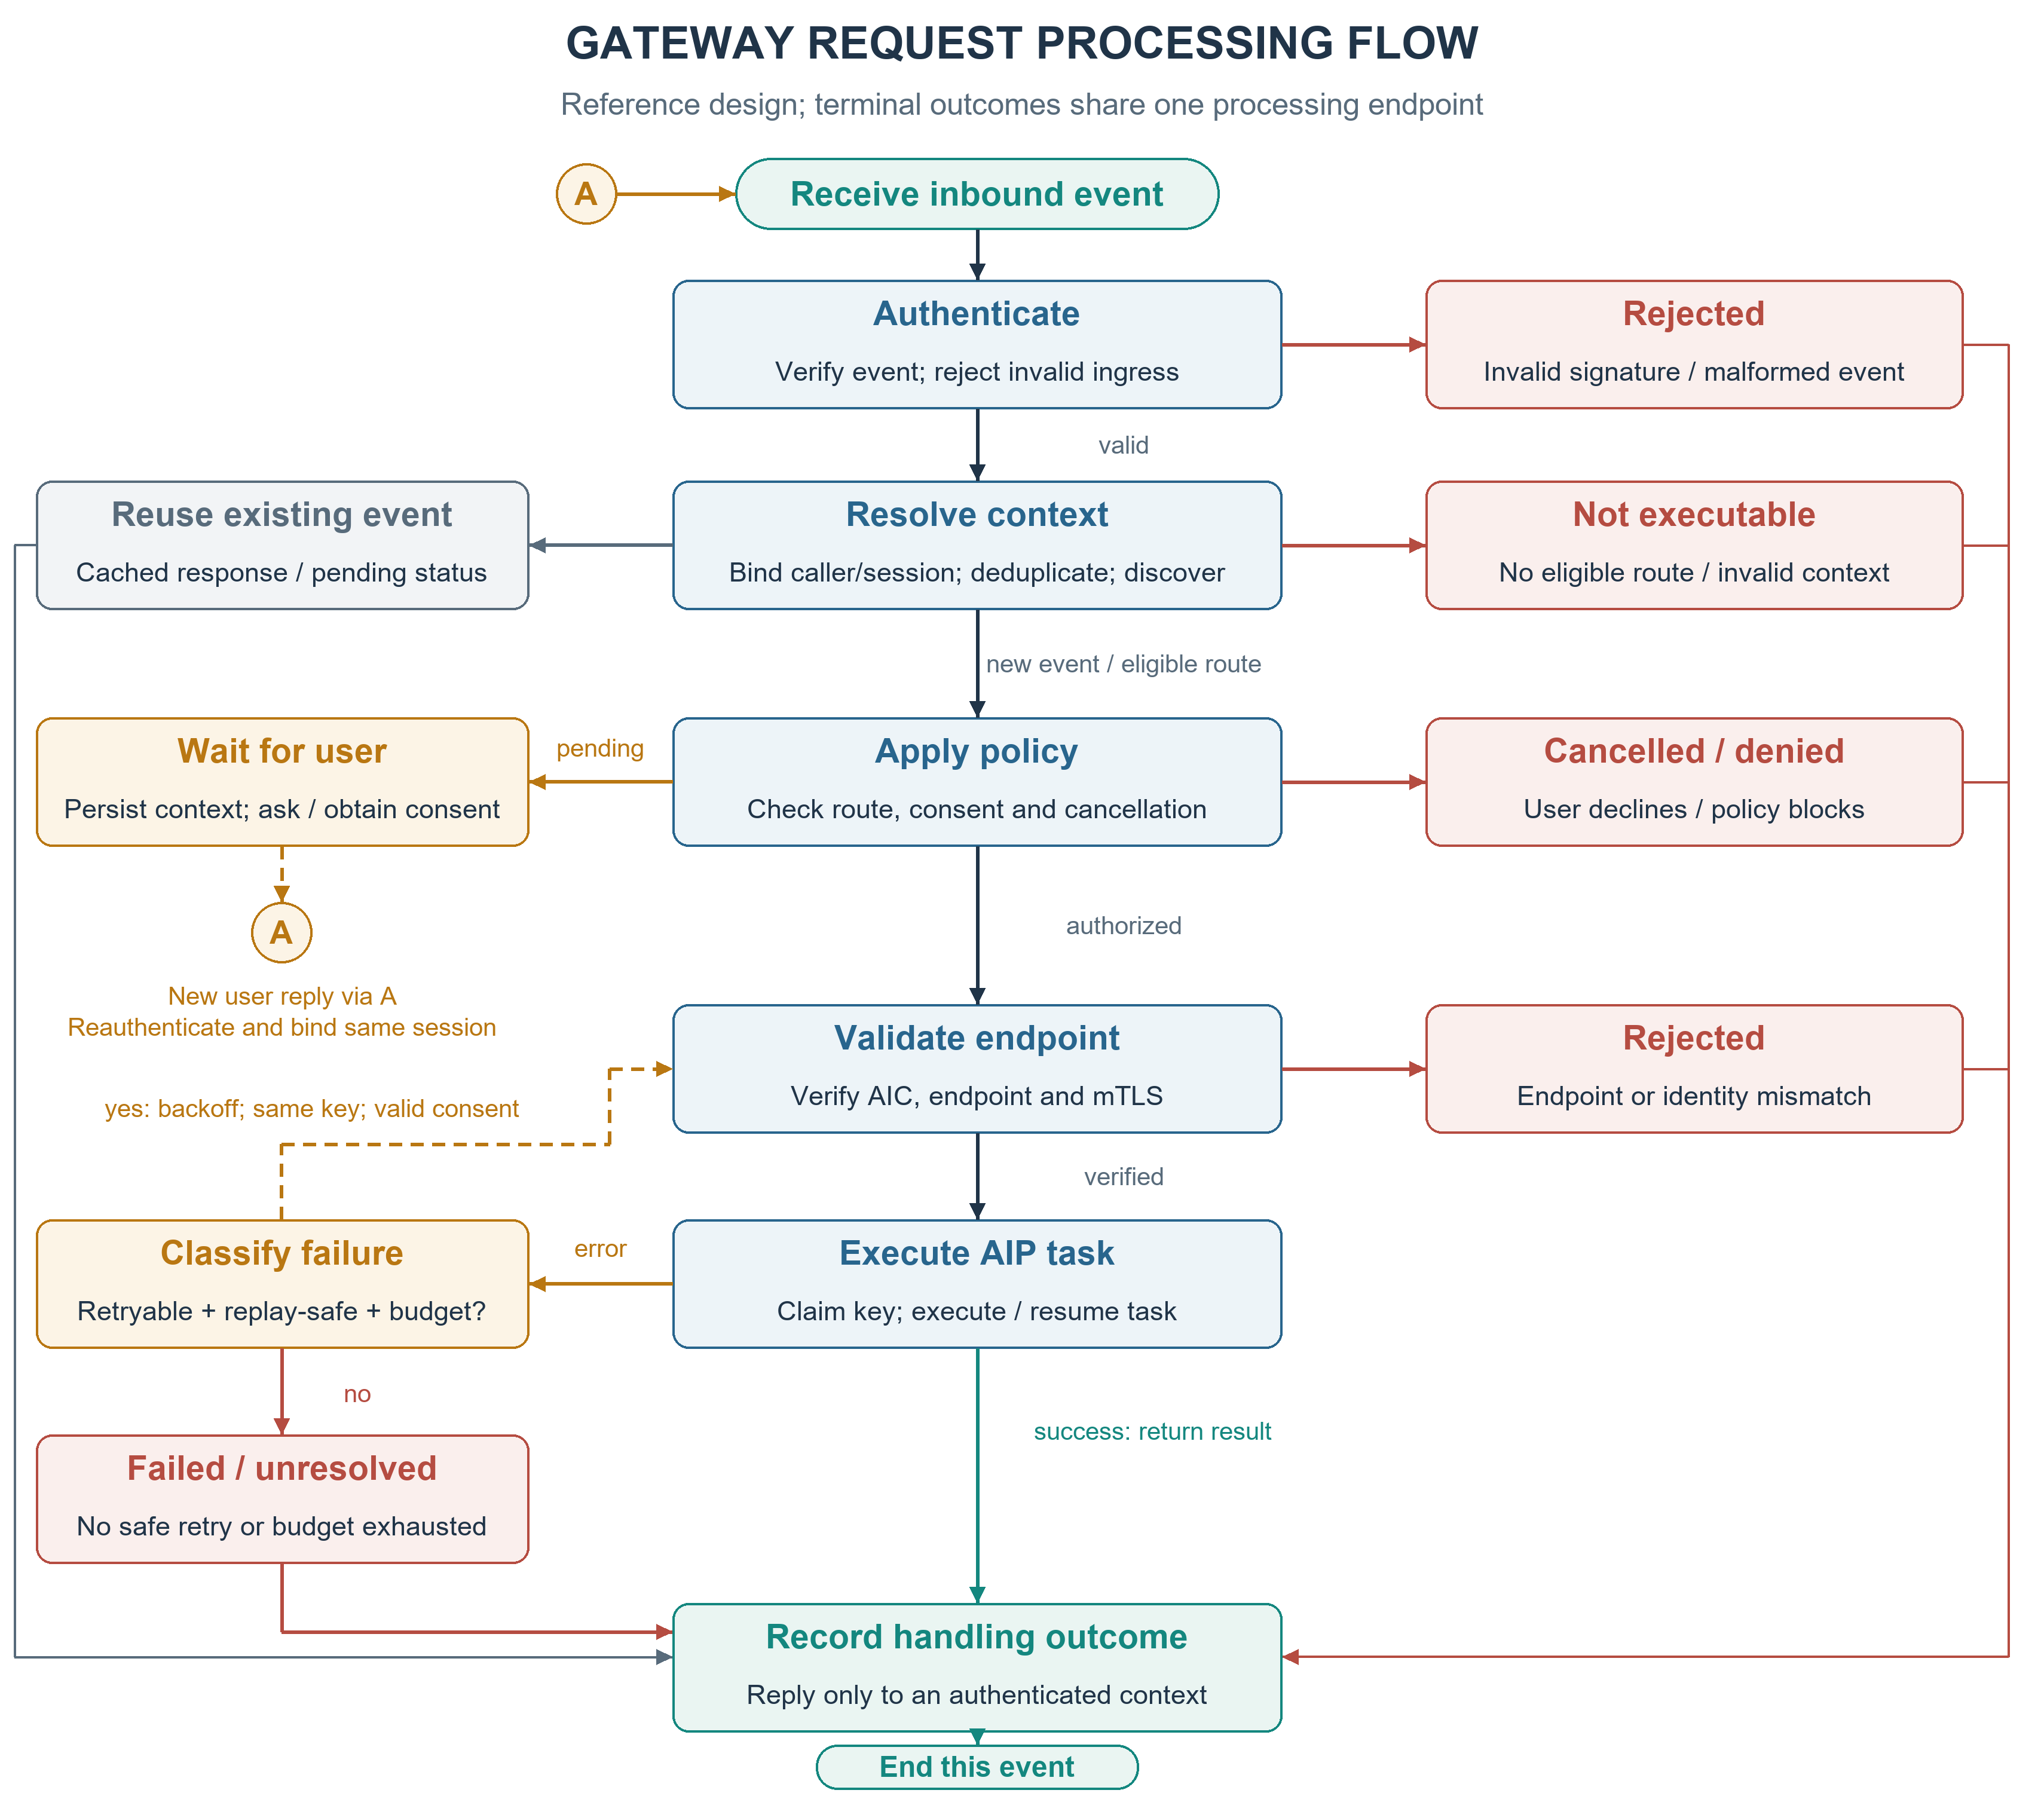
\includegraphics[width=0.60\linewidth]{../figures/fig2_state_machine.png}

\vspace{1mm}
\raggedright
\small\textbf{Figure 2.} Deduplication precedes every model call; a pending
consent re-enters at authentication; a failed identity or endpoint check never
reaches execution.
\end{block}

\end{minipage}\hfill
\begin{minipage}[t]{0.482\textwidth}
\vspace{0pt}

\begin{block}{}
\sectionbar{Results}
\vspace{2mm}
\textbf{Routing.} The generated target was recommended for 48/48/50 of 50
direct requests; 39/38/38 of 40 ambiguous requests received more than one
agent; 0/40 out-of-scope requests recommended a study partner.

\vspace{1.5mm}
\centering
\begin{tabular}{@{}lcc@{}}
\toprule
\textbf{Ablation} & \textbf{Control} & \textbf{Removed} \\
\midrule
Identity binding & 0/30 & 30/30 \\
Caller isolation & 0/30 & 30/30 \\
Idempotency & 30 exec. & 60 exec. \\
\bottomrule
\end{tabular}
\vspace{1.5mm}
\raggedright

\textbf{Consent.} No partner action before consent (0/40); every consent
produced exactly one action (36/36).

\vspace{1.5mm}
\centering
\begin{tabular}{@{}lcc@{}}
\toprule
 & \textbf{Typed} & \textbf{Free text} \\
\midrule
Accuracy & 94.1\% & 83.9\% \\
Brier & 0.095 & 0.266 \\
ECE & 0.026 & 0.144 \\
\bottomrule
\end{tabular}

\vspace{1.5mm}
\raggedright
\small The injection stress set (200 injected, 256 benign near-misses) misses
none but flags about half of quoted mentions, which is why the injection score
only parameterizes policy.

\vspace{2mm}
\centering
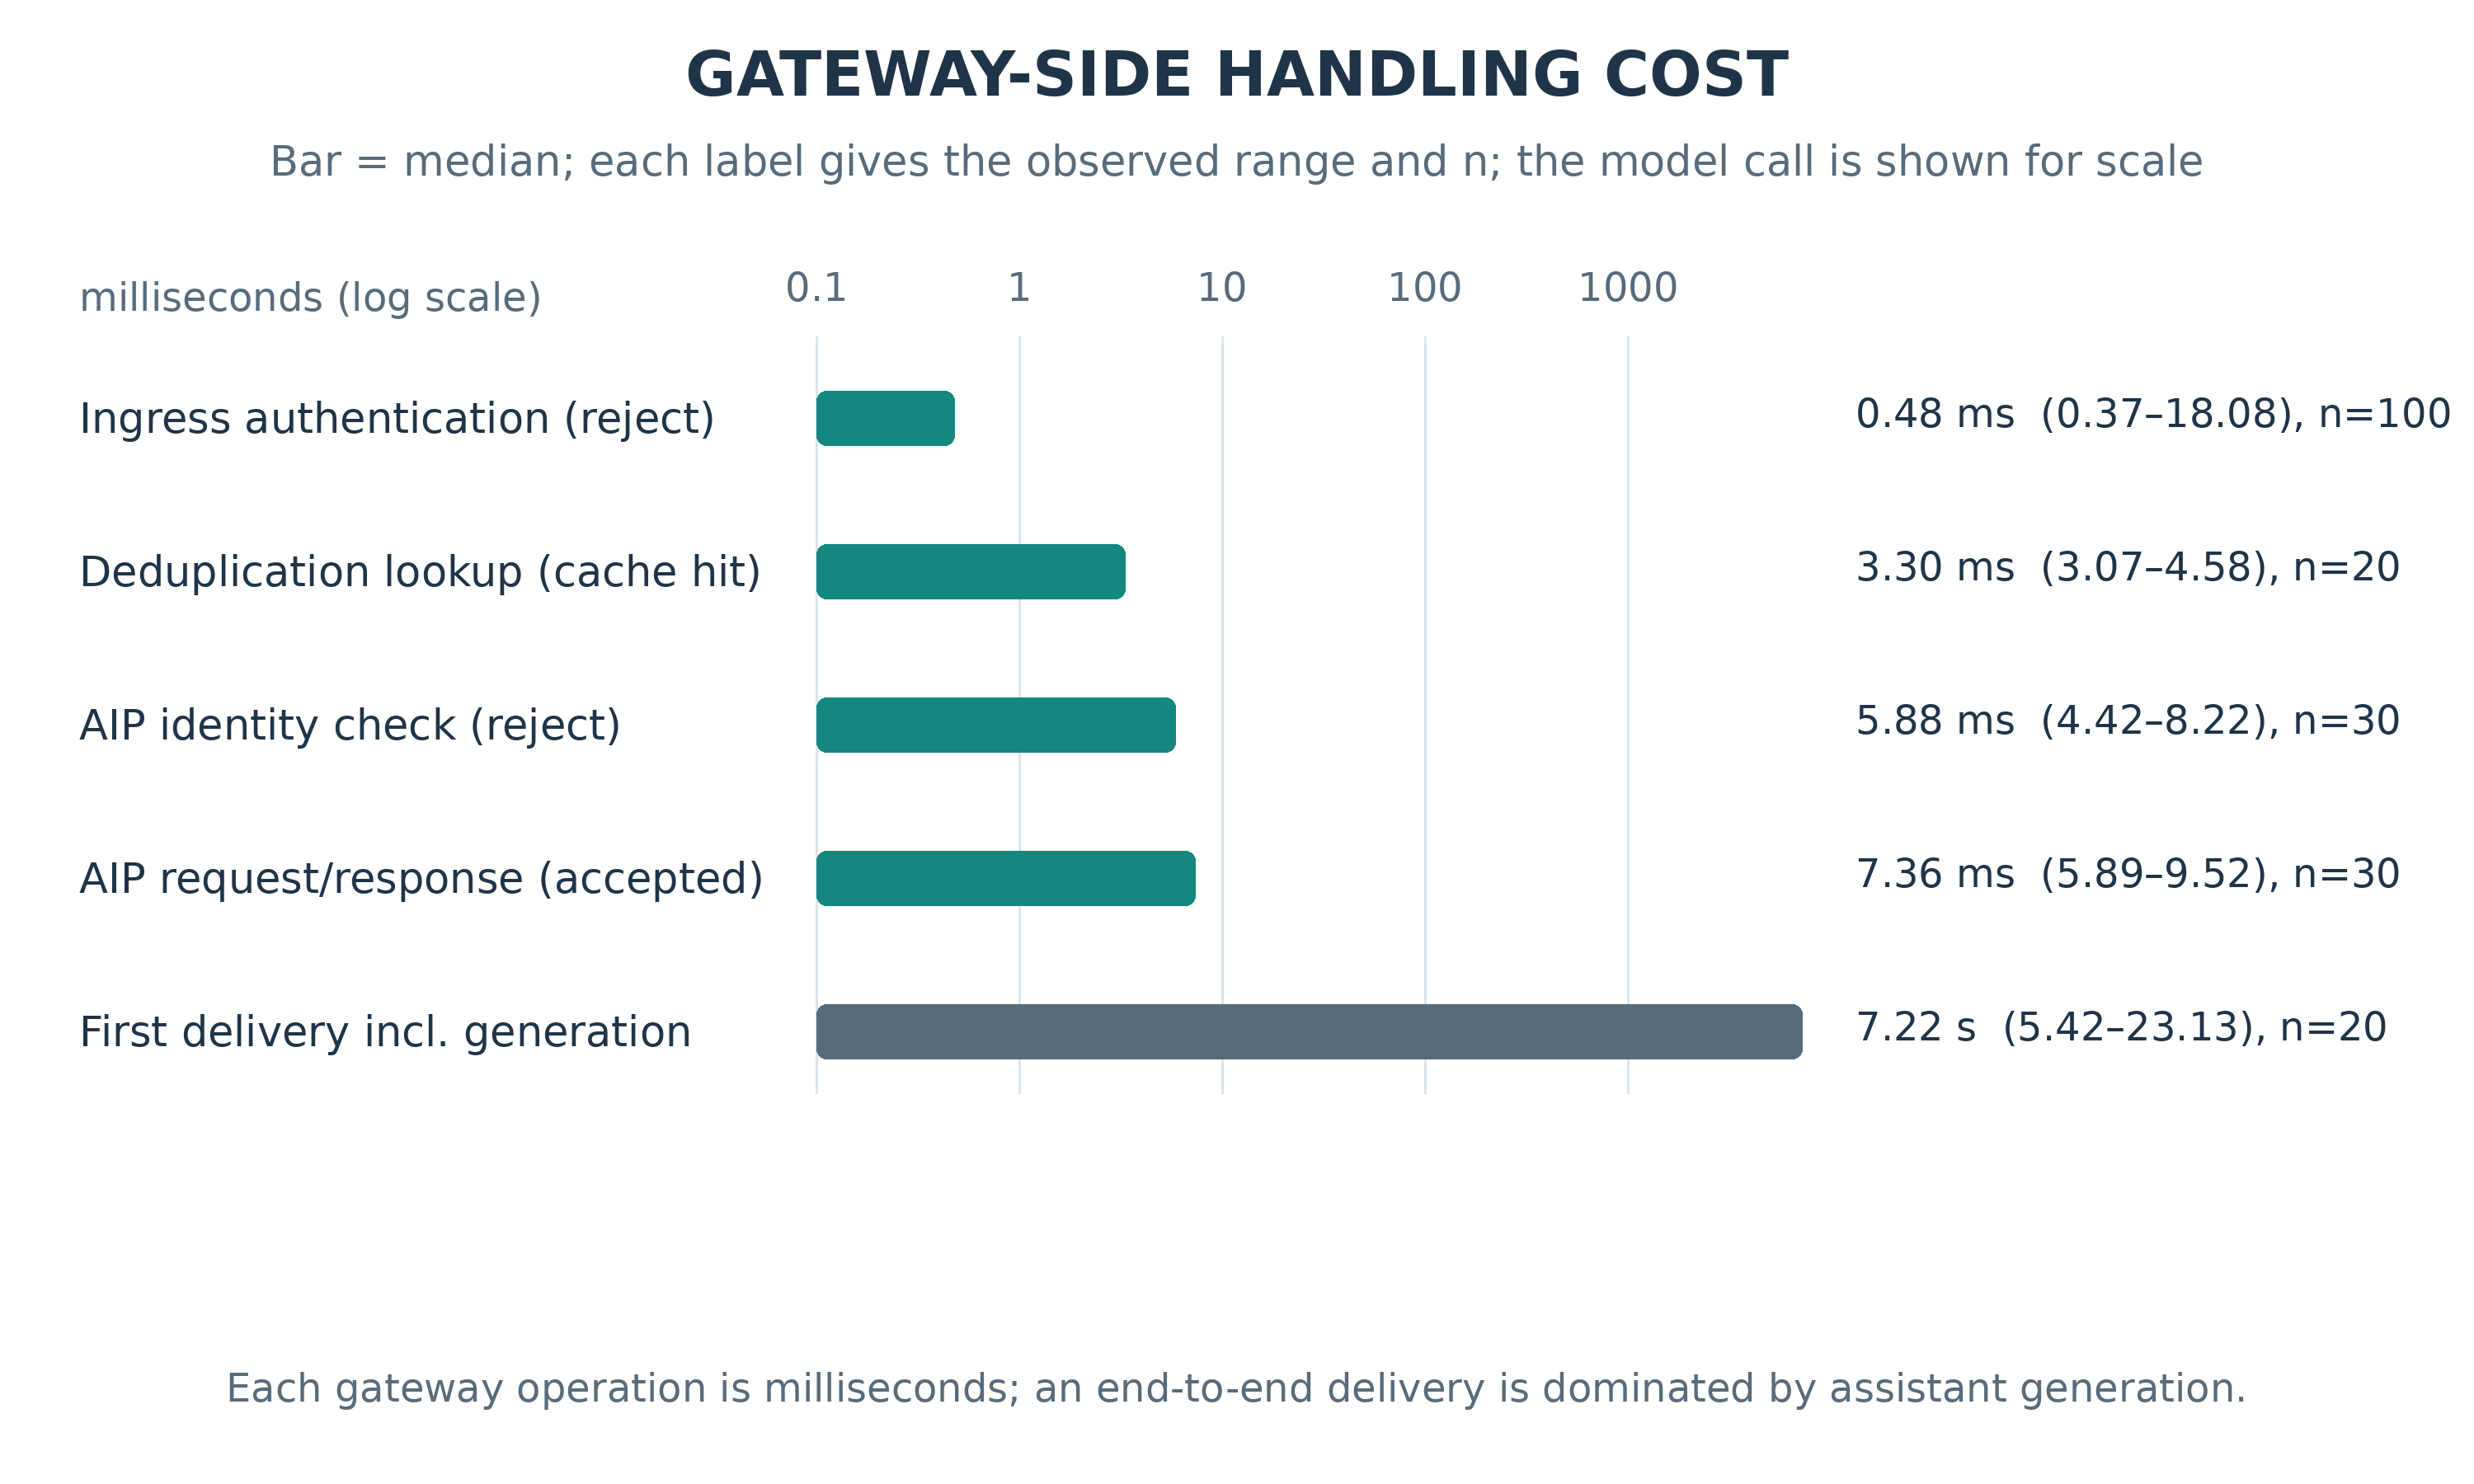
\includegraphics[width=1.0\linewidth]{../figures/fig3_overhead.png}

\vspace{1mm}
\raggedright
\small\textbf{Figure 3.} Median gateway-side handling cost per operation.
\end{block}

\vspace{22mm}

\begin{block}{}
\sectionbar{Conclusion}
\vspace{2mm}
The model advises; code controls identity, state, and every side effect. Typed
answers are more accurate and better calibrated than free text, and consent
gating admits exactly one partner action per accepted event. At a glance:
48/48/50 targets recommended, 0/30 to 30/30 under the identity ablation, 36/36
one-action consents, and 94.1\% versus 83.9\% accuracy.
\end{block}

\vspace{22mm}

\begin{block}{}
\sectionbar{References}
\vspace{1.5mm}
{\small
\mbox{[1]} J. Liu et al., ACPs: Agent Collaboration Protocols for the Internet of Agents, arXiv:2505.13523, 2025.\par
\mbox{[2]} Q. Zhan et al., InjecAgent, arXiv:2403.02691, 2024.\par
\mbox{[3]} S. Chen et al., StruQ, arXiv:2402.06363, 2024.\par
\mbox{[4]} E. Debenedetti et al., AgentDojo, NeurIPS 2024.}
\end{block}

\vspace{22mm}

\begin{block}{}
\sectionbar{Contact}
\vspace{1.5mm}
{\small
Paper RI080\quad\textbar\quad JCRAI 2026, Special Session XII\\
Yizhang Cai, \texttt{2025111259@bupt.cn}\\
Artifact: \texttt{github.com/ankelas/consent-gated-gateway-artifact}\\
Supported by S\&T Program of Xiongan New Area (No. XA2026111001K).}
\end{block}

\end{minipage}

\vspace{4mm}

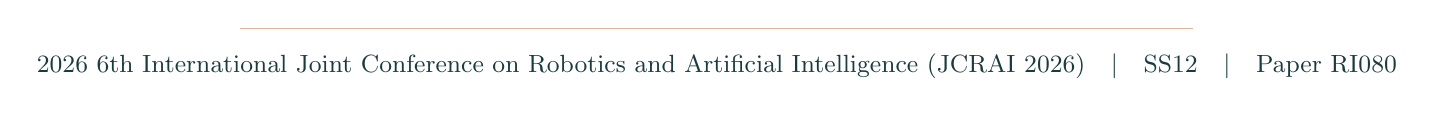
\begin{tikzpicture}
  \draw[rule, line width=0.4pt] (0,0) -- (\dimexpr\textwidth-0.5pt\relax,0);
  \node[anchor=north] at (0.5\textwidth,-2mm)
    {\small\color{ink}2026 6th International Joint Conference on Robotics and
     Artificial Intelligence (JCRAI 2026)\quad\textbar\quad SS12\quad\textbar\quad Paper RI080};
\end{tikzpicture}

\end{document}
